\documentclass[a4paper,twocolumn,10pt]{article}
\usepackage{amsfonts}
\usepackage{amssymb}
\usepackage{amsmath}
\usepackage{latexsym}
\usepackage{cuted}
\usepackage{graphicx}
\usepackage[sorting=none]{biblatex}
\usepackage[skip=2pt, font=scriptsize]{caption}
\usepackage{indentfirst}
\usepackage{enumitem}
\usepackage{mathtools}
\hyphenpenalty1000
\addbibresource{main.bib}
\usepackage{graphicx}  % Required for \includegraphics
% Drawing
\usepackage{tikz}
\usepackage{tikz-3dplot}
% Styles
\tikzset{>=latex}

\newcommand\blfootnote[1]{%
  \begingroup
  \renewcommand\thefootnote{}\footnote{#1}%
  \addtocounter{footnote}{-1}%
  \endgroup
}

% TODO: Add citation for the tilt frame compensation
% TODO: Add workspace analysis
% TODO: 

\begin{document}

\title{Kinematics of X-Y Pedestals
with Joint and Pointing Misalignment } 
\author{Buğra Coşkun\thanks{E-mail:
\texttt{bugra.coskun@profen.com}}
\thanks{ORCID: \texttt{0009-0002-0177-684X}} \\
\multicolumn{1}{p{.3\textwidth}}
{\centering\footnotesize\texttt{Profen Communication Technologies \& 
Services, Inc.}}
}

\date{\vspace{-1ex}\scriptsize26.11.2023}
\maketitle
\vspace{-5ex}
%Technologies \& Services, Inc.}
\normalsize

\begin{abstract}
    We describe the kinematics of X-Y pedestals with unideal geometry caused by
    joint and pointing misalignment that might arise from issues in
    manufacturing, assembly or mechanical wear. We present it's real and
    complex inverse kinematic solutions that are produced through classical
    methods of analysis and test their validity using
    simulations of discrete rotations.
\end{abstract}

\section*{Introduction}
X-Y pedestals are manipulators of two revolute joints ideally positioned
orthogonally with one stacked on top of the other, with both parallel to the
tangent plane of Earth spheroid at that location. They are a popular design
choice for low-earth-orbit satellite tracking applications of high-elevation
passes. They are preferred over the alternative altitude-azimuth pedestals that
suffer the zenith problem at positions closer to the azimuth singularity
\cite{ji2003}. While all serial manipulators have singularities
\cite{gottlieb1986}, For X-Y pedestals the singularity is located at the axis
of the stationary joint. This is a concern only for low elevation applications
which is a rare occurence for satellite communications\cite{willey2000}. X-Y
pedestal kinematics is not as intuitive as their altitude-azimuth counterpart,
but given their popularity previous research delving into their dynamics,
kinematics and control that lessens this property already
exists\cite{tehrani2014}. In this paper we hope to fill the gap for a more
general inverse kinematics solution that considers pedestals with misalignment
issues without the need for resynthesizing the inverse kinematics solution.

\begin{figure}[h]
    \centering
    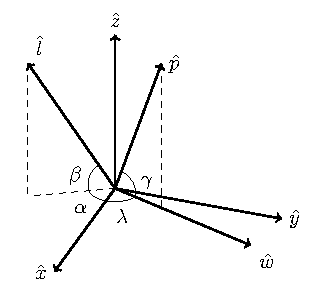
\includegraphics[width=0.4\textwidth]{diagrams}
    %\input[width=0.8\textwidth]{diagrams.tex}
    \caption{Pedestal coordinate system with exagerated misalignments}
    \label{fig:tikzexample}
\end{figure}

For the mathematical model; the stationary joint axis will be deemed the
X-joint and will coincide with $\hat x$ in the pedestal standard basis and it's
rotation angle shall be expressed as $\psi$. For $\psi=0$ the Y-joint axis will
be $\hat w$ at an angle $\lambda$ with $\hat x$ and let $\phi$ be it's rotation
angle. $\hat w$ will belong to the same plane defined by the vectors $\hat x$
and $\hat y$. As such the joint misalignment is $\frac{\pi}{2}-\lambda$. Let
$\hat p$ be the orientation vector at $\psi=0$ and $\phi = 0$. Similar to joint
misalignment, pointing misalignment is $\frac{\pi}{2}-\gamma$. In a real-world
case the pedestal basis should be defined in the NWU or NED frame so as to meet
these definitions. This involves calculating the pedestal $\hat z$ from
positions of pedestal $\hat x$ and $\hat w$ vectors in the selected environment
frame and produce a rotation matrix. This will make it so that any joint
misalignment can be considered using the definitions above. Let the target
orientation be $\hat l$. For inverse kinematics this is usually given as
azimuth and elevation angles and in left-handed spherical coordinates. Taking
the negative of the azimuth angle gives us $\alpha$ and we can produce the
cartesian vector using the appropriate spherical to cartesian mapping.

\normalsize
\section*{Forward Kinematics}
We first consider the rotation around the Y-joint, as Y-joint axis is
modified by the X-joint rotation, this will save us from calculating
the new axis of the Y-joint. This is an example of extrinsic rotation.
\begin{equation}
    \hat w = \begin{bmatrix}
            \cos\lambda \\
            \sin\lambda \\
            0
        \end{bmatrix},
\end{equation}
The skew-symmetric cross product matrix of $\hat w$ is therefore:
\begin{equation}
    W = \begin{bmatrix}
        0 & 0 & \sin\lambda \\
        0 & 0 & -\cos\lambda \\
        -\sin\lambda & \cos\lambda & 0
    \end{bmatrix},
\end{equation}
The rotation matrix for Y-joint in $SO(3)$ group is given by the Rodrigues'
rotation formula:
\begin{equation}
    R_{\hat w}(\phi) = I + (\sin \phi) W + (1 - \cos \phi) W^2,
\end{equation}
The elementary rotation matrix around the $\hat x$ axis is in the form:
\begin{equation}
    R_x ( \psi ) = \begin{bmatrix}
        1 & 0 & 0 \\
        0 & \cos \psi & -\sin \psi \\
        0 & \sin \psi & \cos \psi
    \end{bmatrix},
\end{equation}
We define the orientation vector at initial configuration $\psi = 0$ and $\phi
= 0$ to
be:
\begin{equation}
    \hat p =
    \begin{bmatrix}
        \cos \lambda \cos \gamma\\
        \sin \lambda \cos \gamma\\
        \sin \gamma
    \end{bmatrix},
\end{equation}
Thus the forward kinematic equation becomes:
\begin{equation}
    \hat l = R_{\hat x} ( \psi ) R_{\hat w} ( \phi ) \hat p.
\end{equation}
The resulting line-of-sight vector is in the pedestal frame, which ideally
shall coincide with the North-West-Up frame for our model. Any tilt in the
pedestal frame can be accounted for if we know the orientation of the pedestal
and produce the rotation matrix that gives us the position of pedestal basis
in the NWU frame similar to gimbal calculations for stabilizing the line of 
sight\cite{kaan2018}.
\newpage
\section*{Inverse Kinematics}
For inverse kinematics we introduce the concepts of joint surface and loose
reachability.
We define the surface of a joint as being the set of all unitary vectors where
their dot products against the joint axis are some value $c$.
\begin{equation} 
    c \in (-1,1),\; \mathbb{S}_{\hat k}(c) = \{ \hat v :
        \hat v \cdot \hat k = c \}.
\end{equation}
For any rotation around the joint axis the dot products of vectors belonging
to the surface are conserved:
\begin{equation}
    \begin{split}
        \forall \hat v \in \mathbb{S}_{\hat k}(c)&,\; 
        \forall \theta \in (-\pi,\pi],\\
        R_{\hat k}(\theta)\hat v \in \mathbb{S}_{\hat k}(c)
        &\because R_{\hat k}(\theta) \in SO(3).
    \end{split}
\end{equation}
Following that,
\begin{align}
        \hat l \in \mathbb{S}_{\hat x} (\hat l \cdot \hat x) \;\therefore\;
        &R_{\hat x} (\psi) R_{\hat w}(\phi) \hat p = \hat l \\
        \iff &R_{\hat w}(\phi) \hat p 
        \in \mathbb{S}_{\hat x}(\hat l \cdot \hat x) \\
        \iff &R_{\hat w} (\phi) \hat p \cdot \hat x = 
        \hat l \cdot \hat x.
\end{align}
Thus if $\exists \phi \in (-\pi,\pi]$ such that Eq(9) holds we consider the
position to be loosely reachable (ie. a real solution exists without
considering joint limitations). Solving Eq(10) for $\phi$ we get:

\begin{equation}
    \phi = \sin^{-1} \left[
        \frac{ \cos\alpha \cos\beta - \cos\gamma \cos\lambda }
        { \sin\gamma \sin\lambda }
    \right].
\end{equation}
If the position is not loosely reachable and $sin^{-1}(x)$ is extended into the
complex plane so that it's defined for $||x||>1$ then $\operatorname{Im}(\phi)
\neq 0$. In such a case the complex angles can be used to find the closest
approximate position in the workspace \cite{pohl1990}.

For solving X-Joint angle $\psi$ independently from the $\phi$ angle we
leverage the fact that $\hat p^*$ shall belong to both joint surfaces if a 
proper $\phi$ angle exists,
\begin{equation}
    \hat p^* = R_{\hat w}(\phi) \hat p,
\end{equation}
\begin{equation}
    \hat p^* \in \mathbb{S}_{\hat x}(\hat l \cdot \hat x) 
    \cap \mathbb{S}_{\hat w}(\hat p \cdot \hat w),
\end{equation}
Using this this property we construct the equation that shall consider $\psi$
in isolation from $\phi$,
\begin{align}
        \;R_{\hat x}(\psi)\hat p^* = \hat l 
        & \iff \hat p^* = R_{\hat x}^{-1}(\psi) \hat l\\
        & \iff R_{\hat x}(-\psi) \hat l
        \in \mathbb{S}_{\hat w}(\hat p \cdot \hat w) \\
        & \iff R_{\hat x}(-\psi) \hat l \cdot \hat w = \hat p \cdot \hat w,
\end{align}
From Eq(15) we get the transcendental equation:
\begin{equation}
   \begin{split}
       \cos\psi \sin\alpha \cos\beta \sin\lambda +
       \sin\psi \sin\beta \sin\lambda \\ 
       - \cos\alpha \cos\beta \cos\lambda +
       \cos \gamma = 0,
   \end{split}
\end{equation}
%   \begin{equation}
%       c\psi s\alpha c\beta s\lambda +
%       s\psi s\beta s\lambda \\ 
%       - c\alpha c\beta c\lambda +
%       c \gamma = 0
%   \end{equation}
To solve this we employ Euler's formula and consider $\psi$ in the complex 
plane. With some algebraic manipulation and application of the quadratic
formula we receive the equation for the nearest root: 
\begin{equation}
    \psi = i \log\left(
        \vcenter{\hbox{$\displaystyle
        \frac{
            \begin{split}
                &-(\cos^{2}{\alpha } \cos^{2}{\beta } \\
                &- 2 \cos{\alpha } \cos{\beta } \cos{\gamma } \cos{\lambda } \\
                &+ \cos^{2}{\gamma } + \cos^{2}{\lambda } - 1)^{\frac{1}{2}} \\
                &+ \cos{\alpha } \cos{\beta } \cos{\lambda } - \cos{\gamma }
            \end{split}
        }
        {
            (\sin{\alpha } \cos{\beta } - i \sin{\beta }) \sin{\lambda }
        }$}}
    \right).
\end{equation}

Alternatively (as in some computational cases it may be undesirable to use
complex numbers), through vector analysis we can compare $\hat l$ and $\hat
p^*$ in the plane defined by $\hat x$ using their cross products with $\hat x$ 
and synthesize another $\psi$ equation that way. Incidentally we do not need to
project $\hat l$ and $\hat p^*$ entirely, their rotation angle around the joint
axis will be preserved for their cross product with the joint axis.
\begin{equation}
    \forall c \in (-1, 1),\;
    \forall \hat k;\;
    \forall \hat v, \forall \hat u \in \mathbb{S}_{\hat k}(c),\;
\end{equation}
\begin{equation}
    R_{\hat k}(\theta) \hat v = \hat u \iff
    R_{\hat k}(\theta) ( \hat v \times \hat k) = ( \hat u \times \hat k)
\end{equation}
It is clear that the resulting vector from the cross product of normalized
$\hat p^* \times \hat x$ and $\hat p^* \times \hat x$ vectors will be parallel
to $\hat x$. And will be equivalent if the rotation angle is positive and vice
versa. To find the sign of the angle in left-handed rotation around 
$\hat x$ we use the dot product. Thus the vector equation and it's simplified
trigonometric form are constructed as such:
\begin{equation}
\begin{aligned}
    \psi &= \sin^{-1} 
    \left[ 
        \left(
           \frac{ \hat p^* \times \hat x }{ || \hat p^* \times \hat x || }
           \times
           \frac{ \hat l \times \hat x }{ || \hat l \times \hat x || }
        \right)
        \cdot \hat x
    \right],\\
    \\
    &= \sin^{-1}{\left(
    \vcenter{\hbox{$\displaystyle
    \frac{
        \begin{aligned}
            - (\sin&\gamma \sin\phi \cos\lambda\\
            - &\sin\lambda \cos\gamma) \sin\beta\\
            &+ \sin\alpha \sin\gamma \cos\beta \cos\phi
        \end{aligned}
    }
    {
        \begin{aligned}
            (- \cos^{2}&\alpha \cos^{2}\beta + 1)^{\frac{1}{2}}\\
            [(\sin&\gamma \sin\phi \cos\lambda\\ 
            - &\sin\lambda \cos\gamma)^{2}\\
            &+ \sin^{2}\gamma \cos^{2}\phi]^{\frac{1}{2}}
        \end{aligned}
    }$}}
\right).}
\end{aligned}
\end{equation}

\section*{Simulation of Discrete\\ Rotations}
To verify the produced equations we test their output by comparing the result
of rotations acting on $\hat p$ to the target orientation $\hat l$. To
visualize the process further we rotate $\hat p$ around $\hat w$ first to
produce $\hat p^*$ and then apply the rotation around $\hat x$.

\begin{figure}[h]
  \centering
  
\includegraphics[width=0.5\textwidth]{"img/comp.png"}
  \caption{Simulation of discrete rotations with produced angles}
  \label{fig:discreterotations}
\end{figure}

For the simulation in Figure 2, we apply the parameters
$\alpha=\frac{\pi}{4.5},\; \beta=\frac{\pi}{4},\; \lambda = \frac{\pi}{2.25},\;
\gamma = \frac{\pi}{2.25}$ in radians and we use the complex equation for
calculating the $\psi$ angle. Inverse kinematic results were $\phi \approx
0.556$ and $\psi \approx 0.796 + i 6.287\textsf{e-17}$. We take the real part
of $\psi$. Rotated $\hat p$ and $\hat l$ were identical and no error was
calculated. Simulations show that for $0 < \varepsilon << 1$ (for the
simulation code using Sympy it's been observed that $\varepsilon \approx
\textsf{1e-9}$):
\begin{align}
    || \hat l \cdot \hat x || &< 1 - \varepsilon \\
    \rightarrow \;\;
    \hat l \cdot (\hat R_{\hat x}(\psi)R_{\hat w}(\phi)\hat p)  &>
    1 - \varepsilon
\end{align}
Thus for non-singular values the simulation did not show any signs of 
significant error, as well as for negative elevation values and the zenith.
The simulation has been written in Python using Sympy and Matplotlib. And
angles produced has been cross checked using Octave. 

\newpage
\section*{Conclusion}
Using analytical methods, we produced and, through simulations, verified a more
general inverse kinematics solution for X-Y pedestals that take into account
joint and pointing misalignments.  The inverse kinematics equations have a
relatively low computational complexity and (if the computing environment
supports complex numbers) are robust for out-of-workspace positions. 


\section*{Acknowledgements}
This research has been funded by \textbf{Profen Communication Technologies \&
Services, Inc.} The author is thankful to Mustafa Çelik, Cem Doğan and Kadir
Koca for their guidance on X-Y pedestals, to Merve Güvenç for the inspiring
conversations and to Rızkı Tekay for being the catalyst for this research.

\printbibliography

\end{document}
